\section{Signaling Protocol}

The signaling protocol could be implemented using \ac{HTTP} messages but they would transport extra information such as \ac{HTTP} headers and would follow a request response signaling mechnism which would not be the best option, as multiple ice candidates can arrive at any time. For that reason bi-directional communications were prefered.

Our signaling protocol consists in send and receiving JSON formated messages over WebSockets by both the server and the client. 

\begin{lstlisting}[caption={General structure of our WebSocket messages},language=json]
{
	"cmd":<cmd>,
	"data":<data>
}
\end{lstlisting}

When a user enters in a group conference, after the page is completely loaded it is created a WebSocket that mantains a connection with our web servers. 
Before creating the web socket, we must identify the user and check if he has permissions to participate in the conference. The user identification is done by retrieving the session id from the cookie provided by the user through the \ac{HTTP} headers then we retrieve all the information need from database in order to check if the user has permissions to join the conference room. It's important to save de user identification before the socket is created because after the the handshake performed by the \emph{WebSocket} protocol\cite{rfc6455} the \ac{HTTP} context is lost.

When the connection is established between the server and the client, a \emph{PeerConnection} is created on the client and imediately after an \ac{WebRTC} endpoint on the server specifying a possible set of \ac{ICE} servers to connect.

The user is asked if he whants to share its camera and microphone, share screen or just receive streams from the server. If the user decides to perform a screen share, \emph{adapter.js}\footnote{\url{https://github.com/Temasys/AdapterJS}(accessed March 15, 2015).} may ask to install a pluggin if the browser doesn't support screen sharing.

If the user decides to share either from camera of screen, \emph{getUserMedia} is called with the correspondent contraints in order to obtain a local stream. 

\begin{lstlisting}[caption={Media constraints},language=JavaScript]
var screenShareConstraints = {	
	"video": {
		"mediaSource": "window" || "screen"
	}, 
	"audio": false
};
var cameraMicrophoneConstraints = {
	"audio":true, 
	"video":true 
};
var receiveOnlyConstraints = {
	"offerToReceiveAudio":true,
	"offerToReceiveVideo":true
};
\end{lstlisting}

A popup is raised in order to ask the user to give permission to share those resources. If the resources are shared successfully the user creates an offer, sets a \emph{local session description} to its \emph{PeerConnection} and sends it through WebSockets. If the resources are not shared or the user specified to receive stream only, an offer is created specifying the contraints for receiving only video and audio.

The \emph{local session description} contains the session identifier, codecs, containers, transport protocols and ports used per media type. The \emph{local session description} is useful to conclude if the client is receiving only, which means that \ac{KMS} doesn't need to mix, record and analyse streams coming from the user \ac{WebRTC} endpoint. 

The server receive and processes the offer and sets the \emph{remote session description} to its client associated \ac{WebRTC} endpoint. Then a \emph{local session description} is created on the server and sent back to the client, after that the server trys to gather \ac{ICE} candidates.

The client receives the server answer, sets the \emph{remote session description} and gets the ice candidates from the \ac{ICE} server. 

After a while both the server and client receive the \ac{ICE} candidates that allow the client to connect directly to \ac{KMS} and vice-versa. The candidates are received at the client which sets them to its \emph{PeerConnection}. The same is done on the server which receives the \ac{ICE} candidates from the client and propagates them to \ac{KMS}.

An \ac{ICE} candidate contains an \ac{IP}, port, used transport protocol and an attribute named \emph{sdpMLineIndex} that is used for mapping to the \emph{remote session description} media type.

Both intervenients test the conectivity of each \ac{ICE} candidate. When a connection is established the user and server start to interchange stream data but other \ac{ICE} candidates may arrive with better connections, when that happens the connection changes seamlessly. 

With the media session established, the server starts to record any received stream and the client creates an \ac{URL} correspondent to the stream location.

\begin{figure}[H]
    \centering
    \begin{subfigure}[b]{0.5pc}
    	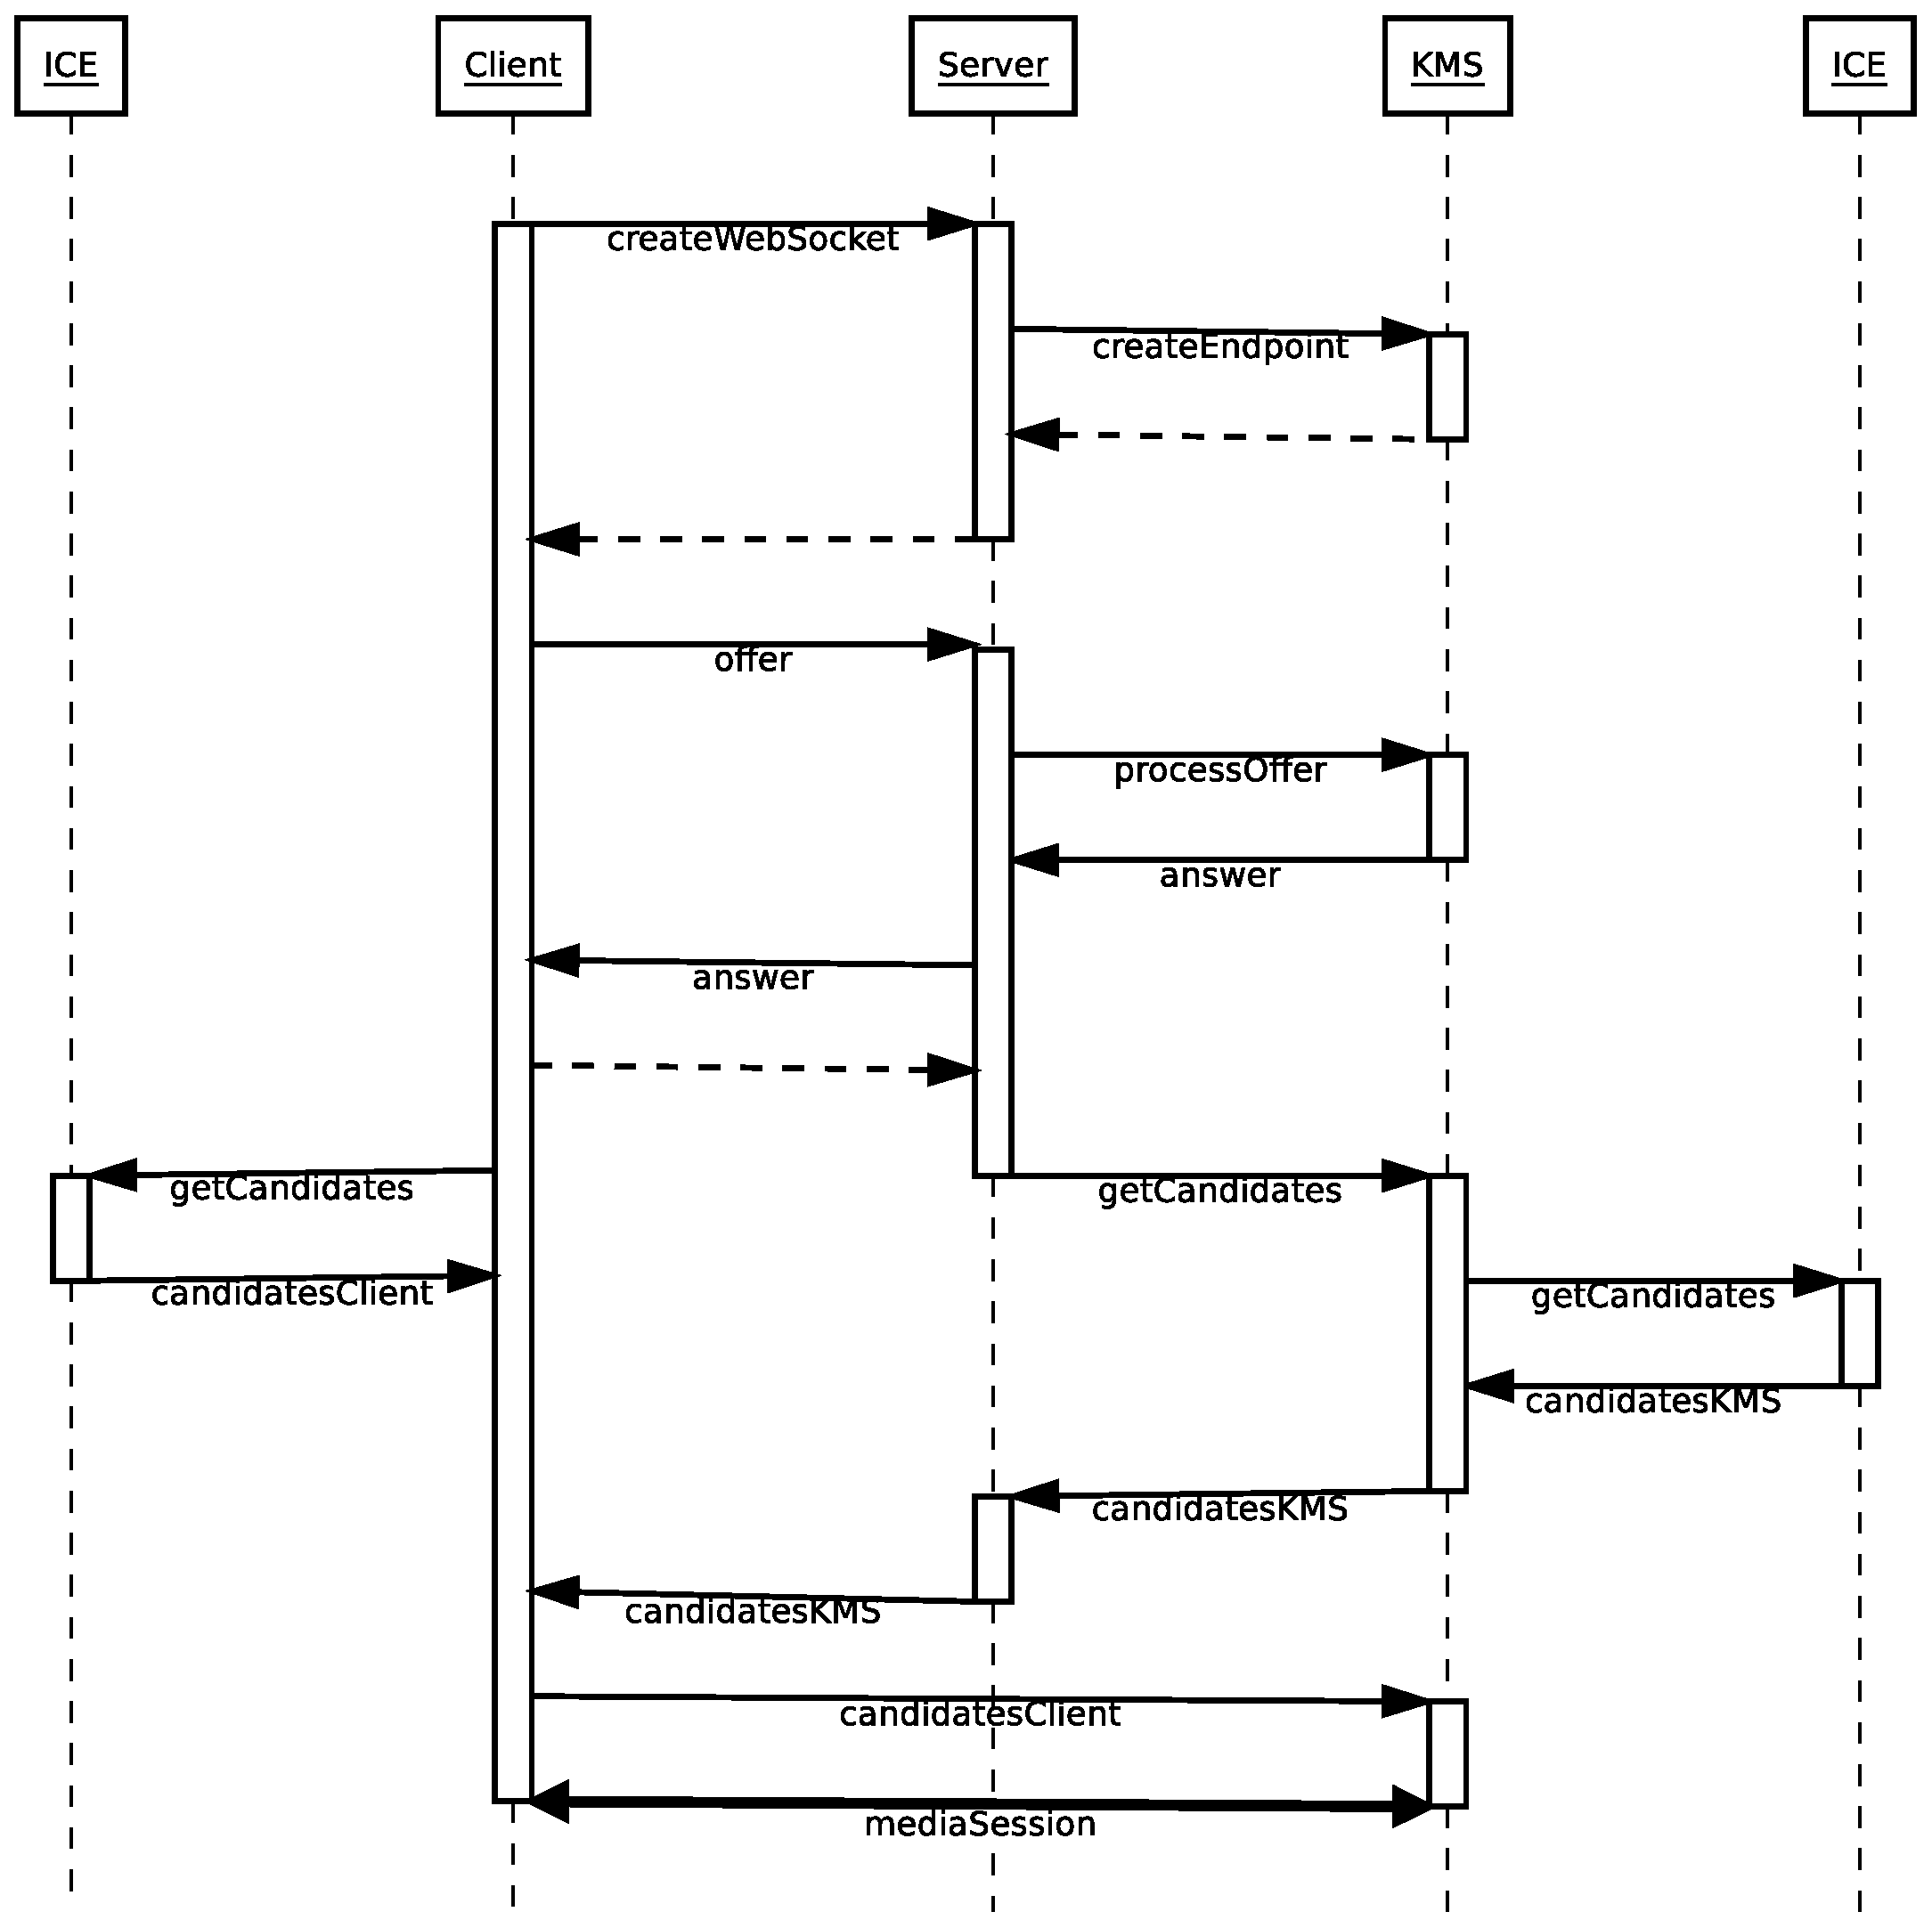
\includegraphics[width=1.0\textwidth]{figures/signaling}
    \end{subfigure}
    \caption{Signaling sequence diagram}
\end{figure} 
